\section{Example Problem}
	\label{s:example problem}
	This section presents an example problem to demonstrate the process of obtaining the FPG and the advantages of doing so. 
	For this example, the algorithm from Sec.~\ref{ss:obtaining FPG} was implemented in the NetworkX package of the Python programming language. 
	While any language with the ability to manipulate graphs is applicable, NetworkX was chosen due to its built-in features, such as cycle detection and shortest path algorithms.

	The example task is to create an FPG for the conceptual sizing of a single-aisle subsonic transport using a set of analysis tools with objectives including performance and gross weight for a required mission. 
	The full set of analysis codes available for use is provided in Table \ref{t:analysis codes}.
	\begin{table}[htbp]
	  \centering
	  \caption{Analysis codes for subsonic transport sizing}
		\begin{tabular}{cc}
		\toprule
		analysis code & description \\
		\midrule
		VSP   & parametric vehicle geometry \\
		PDCYL & wing and fuselage weight estimation \\
		NPSS  & engine sizing and performance \\
		VORLAX & aerodynamics using the vortex lattice method \\
		PMARC & aerodynamics using a low-order panel method \\
		WATE  & engine weight estimation \\
		FLOPSa & mission performance, \\
		  & engine sizing, and weight estimation \\
		FLOPSb & mission performance only \\
		\bottomrule
		\end{tabular}%
	  \label{t:analysis codes}%
	\end{table}%
	Each analysis code contributes individual disciplinary analysis capability, but the outputs of the codes are not mutually exclusive. 
	For example, VORLAX and PMARC are both aerodynamics codes that predict inviscid drag but with different levels of fidelity. 
	The Flight Optimization System (FLOPS) is included twice to represent two different configurations corresponding to different uses. 
	FLOPSa denotes FLOPS implemented to execute both mission performance and engine analysis, while FLOPSb indicates  FLOPS implemented to execute for only mission performance analysis. 
	This representation is useful for ``supercodes'' that are capable of being implemented in different ways and with different sets of inputs and outputs.
The enumeration of these analysis tools and objectives concludes step (A) in Sec.~\ref{ss:process}.

Step (B) is the production of the MCG.
	In this example, the MCG is formed using a consistant variable naming convention and then connecting all variables with the same name with connection edges. 
	Table \ref{t:ins and outs} presents the full list of variables in the leftmost column and indicates whether the variable is an input or an output of each analysis code. 
	Some variables, such as geometry and performance, represent groups of variables that are passed as vectors or other structures due to their similarity. 
	This bundling of variables is not fundamental and does not limit the generality of this example; rather, it simplifies the presentation.
	\begin{table}[htb!]
	  \centering
	  \caption{Analysis code input and output description}
		\begin{tabular}{ccccccccc}
		\toprule
		variable & \multicolumn{8}{c}{analysis code} \\
		\midrule
			  & VSP   & PDCYL & NPSS  & VORLAX & PMARC & WATE  & FLOPSa & FLOPSb \\
		geometry & in    & in    &       & in    & in    & in    & in    & in \\
		number of engines &       &       & in    &       &       &       & in    & in \\
		mission &       &       &       &       &       &       & in    & in \\
		fuselage weight &       & out   &       &       &       &       & in    & in \\
		wing weight &       & out   &       &       &       &       & in    & in \\
		engine weight &       &       &       &       &       & out   & out   & in \\
		wetted area & out   &       &       &       &       &       & in    & in \\
		inviscid drag &       &       &       & out   & out   &       &       & in \\
		drag  &       &       & in    &       &       &       & out   & out \\
		engine performance &       &       & out   &       &       & in    & out   & in \\
		performance &       &       &       &       &       &       & out   & out \\
		total weight &       & in    &       &       &       &       & out   & out \\
		\bottomrule
		\end{tabular}
	  \label{t:ins and outs}
	\end{table}

	In this example, the MCG $M$ is formed in four steps:
	\begin{enumerate}
	\item An analysis block is created for each analysis code using the information in each column of Table \ref{t:ins and outs}. 
	Each analysis block is formed by first creating variable nodes for each input and adding directed edges into a single model node. An edge is directed from this model node into a second model node, which is then directed into variable nodes corresponding to each output. 
	A sample analysis block is shown for analysis code FLOPSa in Fig.~\ref{f:FLOPSb analysis block}.
	\begin{figure}[htb!]
	  \begin{center}
		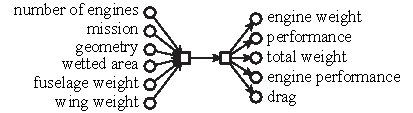
\includegraphics[width=2.75in]{images/FLOPSa_analysis_block}
	  \end{center}
	  \caption{Sample analysis block for analysis code FLOPSa using Table \ref{t:ins and outs}}
	\label{f:FLOPSb analysis block}
	\end{figure}

	\item Expression blocks are created to represent the objectives for performance and total weight.

	\item A variable nodes is created to represent the geometry variable as a global input. Any global inputs incorrectly omitted will be identified in step (D).

	\item Connection edges are created that connect each variable node to every other variable node representing variables with the same name. 
	The direction is determined by whether the variable node has an edge directed into or out of a model node, i.e. whether it is a local input or a local output.
	\end{enumerate}
	The resulting MCG is shown in Fig.~\ref{f:MCG holes}. 
	Cycles are shown as dashed lines. FPGs formed from this MCG may or may not retain these cycles.
	\begin{figure}[htb!]
	  \begin{center}
		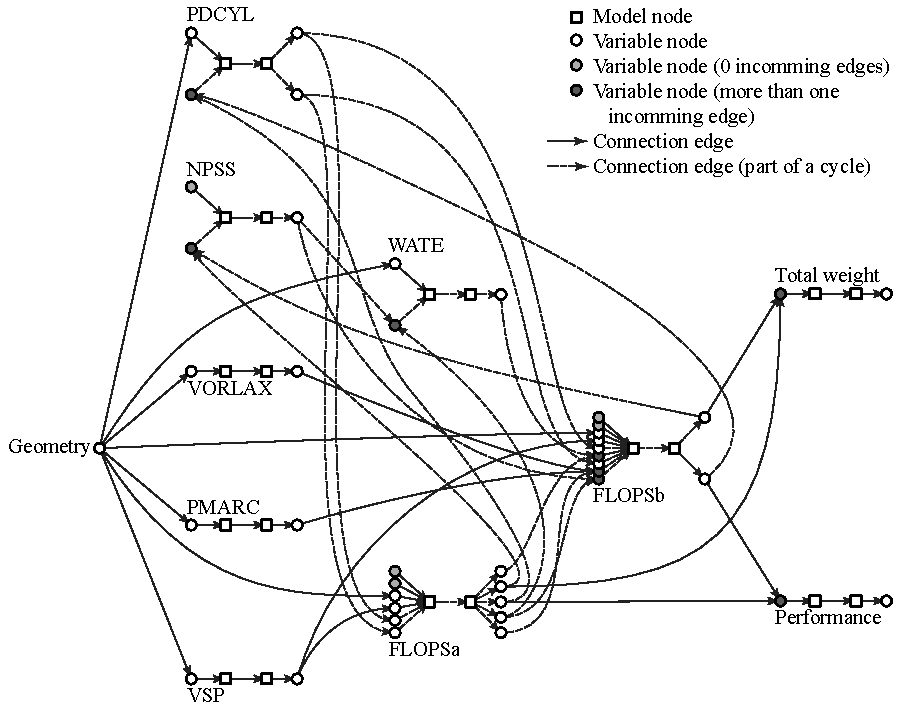
\includegraphics[width=4.5in]{images/MCG_edit_holes}
	  \end{center}
	  \caption{Maximal connectivity graph for the subsonic transport example problem}
	\label{f:MCG holes}
	\end{figure}

To implement step (C) in Sec.~\ref{ss:process}, the indegree of every variable node is set to unity to reflect a single fidelity analysis for which the design variables have not yet been selected.


%	As described in Sec.~\ref{ss:process}, the process of obtaining an FPG from the given MCG is expected to be an iterative process in which the user applies the algorithm to determine whether or not an FPG can be obtained, 
%	and then modifies the indegree limits or the MCG to obtain a satisfactory FPG.
%	For example, after determining the location of a hole, the user can change the indegree limit to make the node a design variable, or the user could change the MCG by adding a new analysis code such that the hole is resolved.
%
%	As presented in Sec.~\ref{s:building graphs}.\ref{ss:obtaining FPG}, the first step to obtaining an FPG is to detect holes. 
%	To begin, we set the lower indegree limit for every node to be unity. 

Step (D) now procededs by executing the FPG algorithm. An FPG cannot be obtained because the variable nodes representing the number of engines are holes for NPSS, FLOPSa, and FLOPSb, and the variable nodes representing the mission definition are holes for FLOPSa and FLOPSb. These holes propagated upstream and created holes in the objectives, thereby preventing a valid FPG.

Step (D)(a) begins to resolve this conflict by creating a global input for the number of engines. In this example, the number of engines was not originally included as a global input to demonstrate how the process responds to this error.
Step (D)(b) then reduces the lower and upper indegree limits for the variable node representing the mission definition to zero, implying that these nodes must be specified as design variables (see Table \ref{t:variable node classification}). The new MCG is shown in Fig.~\ref{f:MCG}.
	\begin{figure}[htb!]
	  \begin{center}
		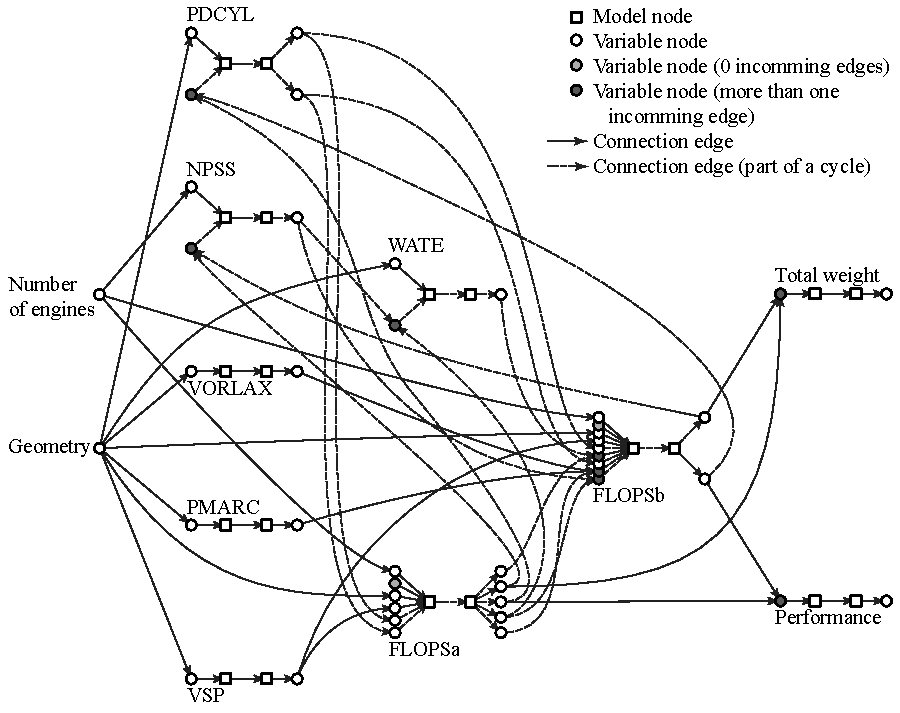
\includegraphics[width=4.5in]{images/MCG_edit}
	  \end{center}
	  \caption{The updated MCG with a new global input.}
	\label{f:MCG}
	\end{figure}

	Although an FPG may now be obtained, this process has not provided a method to decide which edges to retain when resolving a collision, and these decisions will likely determine which analysis tools are included in the FPG. These decisions are left to the discretion of the designer in the context of the specific implementation. 
	However, the graph-based approach presented in this paper enables standard graph algorithms to be employed to automate these decisions based on considerations of metrics related to the graph or other data related to the analysis. 
	An example is a metric to obtain an FPG with the fewest possible number of cycles. 
In this example, the FPG with the fewest number cycles is shown in Fig.~\ref{f:FPG fewest cycles}, in which the edges belonging to a cycle are inticated by dashed lines. 
For this example problem, the cycles were detected using the implementation of Johnson's algorithm \cite{Johnson1975} in the Python package NetworkX. 
There are two cycles which arise from each local output from PDCYL being directed into FLOPSa and then back into PDCYL. 
%((DP:discuss cycle equivalency))
%((mention edge weight for center edge))

	Similar alternatives would be to minimize the number of analysis blocks involved in cycles, counting multiplicity, or to minimize the length of the longest cycle (called the \emph{circumference} of the graph). Since these graphs will always be relatively small (on the order of hundreds of nodes) the 
	computational expense for examining all possible FPGs is negligble compared to the expected expense of using the problem formulation to obtain a solution.
	\begin{figure}[htb!]
	  \begin{center}
		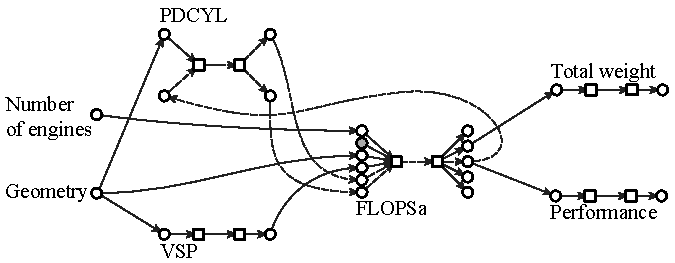
\includegraphics[width=4.5in]{images/FPG_edit_fewest_cycles}
	  \end{center}
	  \caption{FPG with the fewest number of cycles.}
	\label{f:FPG fewest cycles}
	\end{figure}

	Alternatively, it may be desirable to resolve collisions by choosing the higher fidelity analysis tools.
	One method to ensure that the edges directed from certain analysis blocks are those chosen to resolve conflicts is to use a ranking system. Each analysis block is assigned a value by the designer describing how desireable it is for this block to be present in the FPG. The connection edges directed out of each analysis block are then given a weight equal to the value assigned to the analysis block. Finally, each collision is resolved by selected the edges with the highest weights.
For the current example problem, consider the rankings for each analysis code given in Table \ref{t:rankings}.
	\begin{table}[htbp]
	  \centering
	  \caption{Example ranking of importance}
		\begin{tabular}{cc}
		\toprule
		analysis code & rank \\
		\midrule
		VSP   & 5 \\
		PDCYL & 5 \\
		NPSS  & 4 \\
		PMARC & 4 \\
		FLOPSb & 4 \\
		VORLAX & 3 \\
		WATE  & 3 \\
		FLOPSa & 2 \\
		\bottomrule
		\end{tabular}%
	  \label{t:rankings}%
	\end{table}%
	The resulting FPG has four cycles and is shown in Fig.~\ref{f:FPG highest rank}. 
%This graph has four cycles, which are enumerated in Table \ref{t:cycles}.
	\begin{figure}[htb!]
	  \begin{center}
		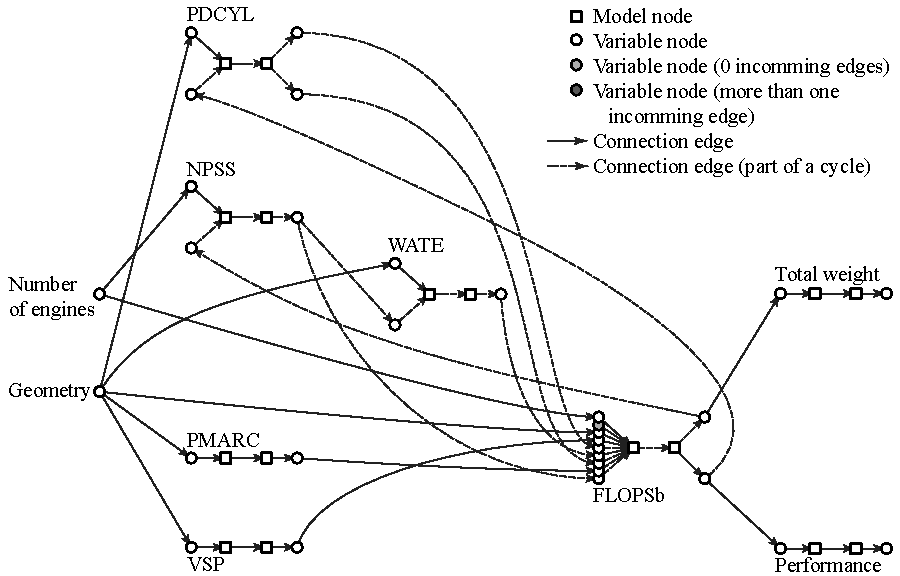
\includegraphics[width=4.5in]{images/FPG_edit_ranking}
	  \end{center}
	  \caption{FPG obtained using the ranking system.}
	\label{f:FPG highest rank}
	\end{figure}
%	\begin{table}[htbp]
%	  \centering
%	  \caption{Cycles for the FPG obtained using ranking}
%		\begin{tabular}{ccccccc}
%		\toprule
%		output/input & analysis code & output/input & analysis code & output/input & analysis code & output/input \\
%		\midrule
%		engine weight & FLOPSb & drag  & NPSS  & engine performance & WATE  & engine weight \\
%		engine performance & FLOPSb & drag  & NPSS  & engine performance &       &  \\
%		fuselage weight & FLOPSb & total weight & PDCYL & fuselage weight &       &  \\
%		wing weight & FLOBSb & total weight & PDCYL & wing weight &       &  \\
%		\bottomrule
%		\end{tabular}%
%	  \label{t:cycles}
%	\end{table}%

	Finally, consider a case in which 
the inviscid drag input into FLOPSb is a multi-fidelity input, meaning that 
 multiple analysis codes calculate the same variable. 
	This multi-fidelity formulation is implemented by setting the upper indegree limit for this node as two and then repreating the (automated) process. 
	In this case, both VORLAX and PMARC are retained, resulting in an FPG that omits only FLOPSa.

